\documentclass[10pt,a4paper, margin=1in]{article}
\usepackage{fullpage}
\usepackage{amsfonts, amsmath, pifont}
\usepackage{amsthm}
\usepackage{graphicx}

\usepackage{tkz-euclide}
\usepackage{tikz}
\usepackage{pgfplots}
\pgfplotsset{compat=1.13}

\usepackage{geometry}
 \geometry{
 a4paper,
 total={210mm,297mm},
 left=10mm,
 right=10mm,
 top=10mm,
 bottom=10mm,
 }
 % Write both of your names here. Fill exxxxxxx with your ceng mail address.
 \author{
  Simsek, Halit \\
  \texttt{e2099760@ceng.metu.edu.tr}
  \and
  Yesilyurt, Yavuz Selim \\
  \texttt{e2259166@ceng.metu.edu.tr}
}
\title{CENG 384 - Signals and Systems for Computer Engineers \\
Spring 2018-2019 \\
Written Assignment 4}
\begin{document}
\maketitle



\noindent\rule{19cm}{1.2pt}

\begin{enumerate}

\item 
    \begin{enumerate}
    % Write your solutions in the following items.
    \item Difference equation of the block diagram is: \\
    \\
    $y[n] = 2x[n] + \frac{3}{4}y[n-1] - \frac{1}{8}y[n-2]$ \\
    
    \item In order to find frequency response, let $x[n]$ to be $e^{jwn}$ so: \\
    \\
    $x[n] = e^{jwn}$ \\
    \\
    $y[n] = H(e^{jw}) \times e^{jwn}$ \\
    \\
    $y[n-1] = H(e^{jw}) \times e^{jw(n-1)}$ \\
    \\
    $y[n-2] = H(e^{jw}) \times e^{jw(n-2)}$ \\
    \\
    Applying above equations to the difference equation: \\
    \\
    $8H(e^{jw})e^{jwn} + H(e^{jw})e^{jwn}e^{-2jw} - 6H(e^{jw})e^{jwn}e^{-jw} = 16e^{jwn}$ \\
    \\
    $H(e^{jw}) = \dfrac{16}{8 + e^{-2jw} - 6e^{-jw}}$ \\
    \\
    \item Let $s = e^{-jw}$ \\
    \\
    $H(e^{jw}) = \dfrac{16}{s^2 -6s + 8} = \dfrac{8}{s-4} - \dfrac{8}{s-2}$ \\
    \\
    Rearranging the above equation: \\
    \\
    $H(e^{jw}) = -2\dfrac{1}{1 - \frac{1}{4}s} + 4\dfrac{1}{1 - \frac{1}{2}s}$ \\
    \\
    Using Fourier Transform lookup table, impulse response becomes: \\
    \\
    $h(n) = [-2(\frac{1}{4})^n + 4(\frac{1}{2})^n]u[n]$
    \\
    
    \item Finding Fourier Transform of the given input: \\
    \\
    $F\{x[n]\} = X(e^{jw}) = \dfrac{1}{1 - \frac{1}{4}e^{-jw}} = \dfrac{4}{4 - s}$ \\
    \\
    Finding output: \\
    \\
    $Y(e^{jw}) = H(e^{jw}) X(e^{jw})$ \\
    \\
    $Y(e^{jw}) = \left(\dfrac{8}{s-4} - \dfrac{8}{s-2}\right) \left( \dfrac{-4}{s-4} \right)$ \\
    \\
    Doing multiplication and using partial fraction expansion we have the following result: \\
    \\
    $Y(e^{jw}) = \dfrac{16}{s-4} - \dfrac{32}{(s-4)^2} - \dfrac{16}{s-2}$ \\
    \\
    Using inverse Fourier Transform we get: \\
    \\
    $y[n]$ = $\left( -4(\frac{1}{4})^n - 2(n + 1)(\frac{1}{4})^n + 8(\frac{1}{2})^n \right)u[n]$ \\
    \\
    $y[n]$ = $\left( -2(n + 3)(\frac{1}{4})^n + 8(\frac{1}{2})^n \right)u[n]$ \\    
    \end{enumerate}


\item Overall impulse response can be represented as:
    \begin{align*}
    h[n] = h_1[n] + h_2[n]
    \end{align*}
    Overall frequency response can be represented as:
    \begin{align*}
    H(e^{jw}) = H_1(e^{jw}) + H_2(e^{jw})
    \end{align*}
    Finding frequency response of $h_2[n]$ and subtracting it from overall frequency response yields $h_1[n]$. So:
    \begin{align*}
    h_1[n] &= \left(\frac{1}{3}\right)^n u[n] \\
    F\{h_1[n]\} &= H_1(e^{jw}) = \dfrac{1}{1 - \frac{1}{3}e^{-jw}}
    \end{align*}
    Subtracting $H_1(e^{jw})$ from overall frequency response yields $H_2(e^{jw})$, so:
    \begin{align*}
    H_2(e^{jw}) &= H(e^{jw}) - H_1(e^{jw}) \\ \\
    &= \dfrac{5e^{-jw} - 12}{e^{-2jw} - 7e^{-jw} + 12} - \dfrac{1}{1 - \frac{1}{3}e^{-jw}} \\ \\
    &= \dfrac{5e^{-jw} - 12}{(e^{-jw} - 3)(e^{-jw} - 4)} + \dfrac{3}{(e^{-jw} - 3)} \\ \\
    &= \dfrac{8}{(e^{-jw} - 4)} \\
    \end{align*}
    Taking Inverse Fourier Transform of $H_2(e^{jw})$, yields $h_2[n]$. So:
    \begin{align*}
    H_2(e^{jw}) &= \dfrac{8}{(e^{-jw} - 4)} = \dfrac{-2}{1 - \frac{1}{4}e^{-jw}} \\
    F^{-1}\{H_2(e^{jw})\} &= h_2[n] = -2\left( \dfrac{1}{4} \right)^n u[n]
    \end{align*}
\item      
    \begin{enumerate}
    \item Finding Fourier Transform of given input: \\
    \\
    \begin{align*}
    x(t) &= x_1(t) + x_2(t) \\
    x_1(t) &= \dfrac{sin(2\pi t)}{\pi t} \\
    F\{x_1(t)\} &= X_1(jw) = \begin{cases}
                               1, & \text{if}\ |w| < 2\pi \\
                               0, & \text{otherwise}
                             \end{cases} \\
    \\
    x_2(t) &= cos(3\pi t) \\
    F\{x_2(t)\} &= X_2(jw) = \pi (\delta (w - 3\pi) + \delta (w + 3\pi)) \\
    \\
    F\{x(t)\} &= X(jw)= X_1(jw) + X_2(jw) \\
    \end{align*}
    We can plot the Fourier transform of the given input as: \\
    \\
\begin{figure}[h!]
    \centering
        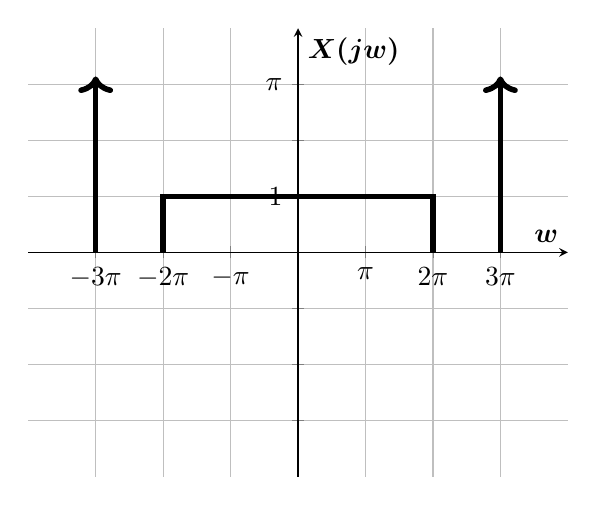
\begin{tikzpicture}[scale=1.0]
           \begin{axis}[
          axis lines=middle,
          xlabel={$\boldsymbol{w}$},
          ylabel={$\boldsymbol{X(jw)}$},
          xtick={-3, ..., 3},
          xticklabels={$-3\pi$, $-2\pi$, $-\pi$, $0$, $\pi$, $2\pi$, $3\pi$},
          yticklabels={, , , , 1, , $\pi$},
          ytick={-3, -2, ..., 3},
          ymin=-4, ymax=4,
          xmin=-4, xmax=4,
          %every axis x label/.style={at={(ticklabel* cs:1.05)}, anchor=west,},
          %every axis y label/.style={at={(ticklabel* cs:1.05)}, anchor=south,},
          grid,
        ]
           \path[draw,line width=2pt] (-2,0) -- (-2,1) -- (2,1) -- (2,0);
           \draw[->, line width=2pt] (-3, 0) -- (-3, 3.14);
           \draw[->, line width=2pt] (3, 0) -- (3, 3.14);
           \end{axis}
        \end{tikzpicture}
        \caption{$w$ vs. $X(jw)$.}
        %\label{fig:q2}
    \end{figure}

    
    \item Nyquist period for sampling is equal to two times of given input's period. Let $w_s$ is sampling period, $T_s$ is sampling frequency and $w_m$ is given input's period.\\
    \\
    $w_m = 3\pi$ \\
    $w_s = 2w_m = 6\pi$ \\
    \\
    $T_s = \dfrac{2\pi}{w_s} = \dfrac{1}{3}$ \\
    
    \item We can directly use the sampling formula which is: \\
    \begin{align*}
    X_p(jw) &= \dfrac{1}{T}\sum_{k = - \infty}^{\infty} X(j(w - kw_s)) \\
    &= X_p(jw) = 3 \sum_k X(j(w - 6\pi k))
    \end{align*}
    Let us plot $X_p(jw)$ and see what it corresponds to: \\
    \begin{figure}[h!]
    \centering
        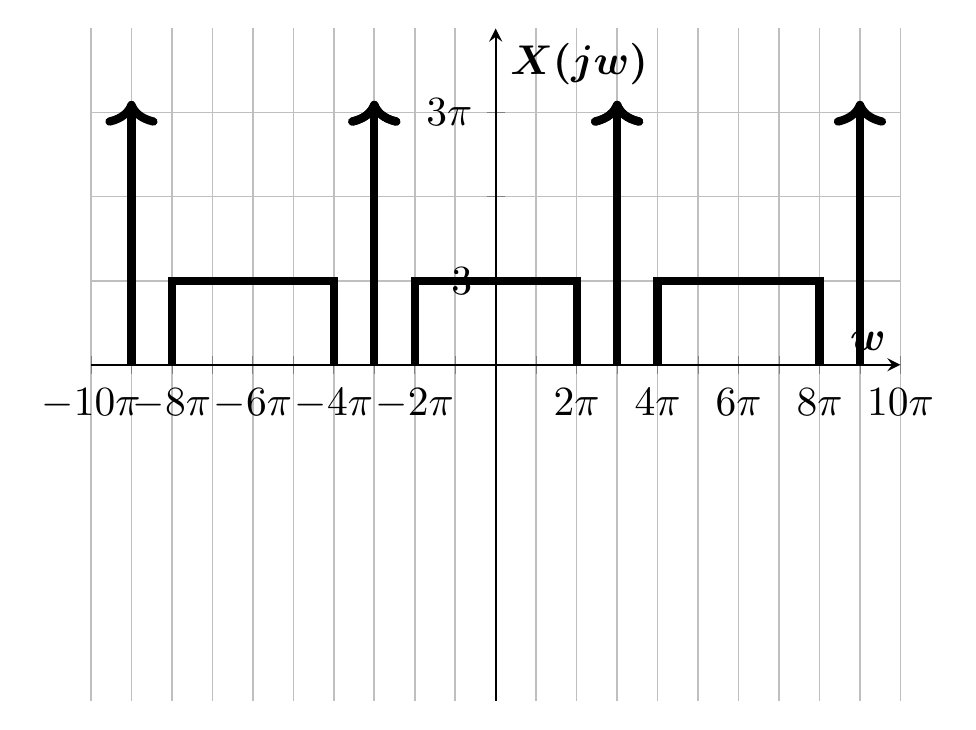
\begin{tikzpicture}[scale=1.5]
           \begin{axis}[
          axis lines=middle,
          xlabel={$\boldsymbol{w}$},
          ylabel={$\boldsymbol{X(jw)}$},
          xtick={-10, ..., 10},
          xticklabels={$-10\pi$, , $-8\pi$, , $-6\pi$, , $-4\pi$, , $-2\pi$, , 0, , $2\pi$, , $4\pi$, , $6\pi$, , $8\pi$, , $10\pi$},
          yticklabels={$0$,$3$,$ $ , $3 \pi$},
          ytick={0,..., 3},
          ymin=-4, ymax=4,
          xmin=-10, xmax=10,
          grid,
        ]
           \path[draw,line width=2pt] (-2,0) -- (-2,1) -- (2,1) -- (2,0);
           \draw[->, line width=2pt] (-3, 0) -- (-3, 3.14);
           \draw[->, line width=2pt] (3, 0) -- (3, 3.14);
           
           \path[draw,line width=2pt] (4,0) -- (4,1) -- (8,1) -- (8,0);
           \draw[->, line width=2pt] (3, 0) -- (3, 3.14);
           \draw[->, line width=2pt] (9, 0) -- (9, 3.14);
           
           \path[draw,line width=2pt] (-4,0) -- (-4,1) -- (-8,1) -- (-8,0);
           \draw[->, line width=2pt] (-3, 0) -- (-3, 3.14);
           \draw[->, line width=2pt] (-9, 0) -- (-9, 3.14);
           
           
           \end{axis}
        \end{tikzpicture}
        \caption{$w$ vs. $X(j(w-6\pi k))$.}
        \label{fig:q3}
    \end{figure}    
    
    \end{enumerate}

\item 
    \begin{enumerate}
    \item Let us first sample $X(jw)$ with an impulse train $p(t) = \sum_{k = - \infty}^{\infty} \delta (t - kT)$. \\

    Sampling period of the input signal can be shown as: \\
    \begin{align*}
    T = \dfrac{2\pi}{w_s} = 2
    \end{align*}
    
    Let $X_p$ represent sampled version of $X(jw)$. So:
    \begin{align*}
    X_p(jw) = \dfrac{1}{T}\sum_{k = - \infty}^{\infty} X(j(w - kw_s))
    \end{align*}
    
    Now we can normalize $X_p(jw)$ as $X_d(e^{jw})$ as the following:
    \begin{align*}
    X_d(e^{jw}) &= X_p(j\dfrac{w}{T}) \\
                &= \begin{cases}
                       \frac{2w}{\pi}, & \text{if}\ |w| < \frac{\pi}{2} \\
                       0, & \text{otherwise}
                   \end{cases} 
    \end{align*}
    \begin{center}
    where $X_d(e^{jw}) = X_d(e^{j(w + N)})$. \\
    \end{center}
	Let $X_d(e^{jw})$ represent discrete version of $X(jw)$. So:
    \begin{align*}
    X_d(e^{jw}) = \sum_{k = - \infty}^{\infty} X\left( \dfrac{j(w - 2k\pi)}{T} \right)
    \end{align*}
   
    \item We know that $h[n] = cos(\pi n) = \frac{1}{2}(e^{j\pi n} + e^{-j\pi n})$ is periodic and we know that $F(e^{jwn}) \leftrightarrow 2\pi \sum_{-\infty}^{\infty} \delta(w-w_0-2\pi k)$, therefore we can proceed as the following: \\
    \begin{align*}
    H(e^{jw}) &= \frac{1}{2} \left( 2\pi \sum_{k = - \infty}^{\infty} \delta (w - \pi -2\pi k) + 2\pi \sum_{k = - \infty}^{\infty} \delta (w + \pi - 2\pi k) \right) \\
    &= \pi \left( \sum_{k = - \infty}^{\infty} \delta (w - \pi - 2\pi k) + \delta (w + \pi - 2\pi k) \right)
    \end{align*}
    
    \item We know that multiplication in time domain corresponds to convolution in frequency domain. Therefore we will convolute $X_d(e^{jw})$ and $H(e^{jw})$ over 1 period (which is 2$\pi$, so use $-\pi \ \text{to} \ \pi$). This can be done with shifting $X_d(e^{jw})$ by $\pi$ to both sides: \\
    \begin{align*}
    y_d[n] &= x_d[n] h[n] \leftrightarrow Y_d(e^{jw}) = \dfrac{1}{2\pi}X_d(e^{jw}) * H(e^{jw}) \\
    &= \begin{cases}
        \frac{w}{\pi}, & \text{if}\ \frac{\pi}{2} \leq |w| \leq \frac{3\pi}{2} \\
        0, & \text{otherwise}
    \end{cases}
    \end{align*}
    \begin{center}
    where $Y_d(e^{jw}) = X_d(e^{j(w + 2\pi)})$.
    \end{center}
    \end{enumerate}

\end{enumerate}
\end{document}

